
\documentclass{standalone}
\usepackage[T1]{fontenc}
\usepackage[utf8]{inputenc}
\usepackage{pgf,tikz}
\usepackage{amsmath}

\newcommand*{\shift}{\ensuremath{\operatorname{q}}}
\begin{document}

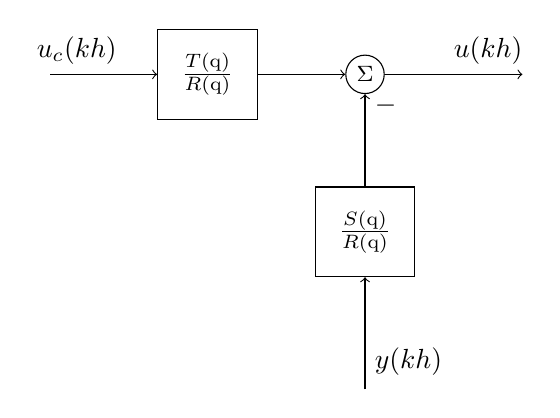
\begin{tikzpicture}[node distance=20mm, anchor=north]
   \node[coordinate] (input) {};
   \node[rectangle, draw, right of=input, inner sep=3mm] (lti) {$\frac{T(\shift)}{R(\shift)}$};
   \node[circle, draw, inner sep=2pt, right of=lti] (sum) {\footnotesize $\Sigma$};
   \node[rectangle, draw, below of=sum, inner sep=3mm] (lti2) {$\frac{S(\shift)}{R(\shift)}$};
   \node[coordinate, right of=sum] (output) {};
   \node[coordinate, below of=lti2] (input2) {};
   \draw[->] (input) -- node[near start, above] {$u_c(kh)$}  (lti);
   \draw[->] (input2) -- node[near start, right] {$y(kh)$}  (lti2);
   \draw[->] (sum) -- node[near end, above] {$u(kh)$} (output);
   \draw[->] (lti) -- node[near end, above] {} (sum);
   \draw[->] (lti2) -- node[very near end, right] {$-$} (sum);
   
 \end{tikzpicture}
\end{document}
